\section{整体设计}
    \subsection{CPU整体设计}
        CPU元件例化独立的模块,
        同时对各个模块的异常与状态信息进行收集,
        决定主状态机的跳转。

        \begin{figure}[!hbp]
            \centering
            \caption{CPU整体设计图}
            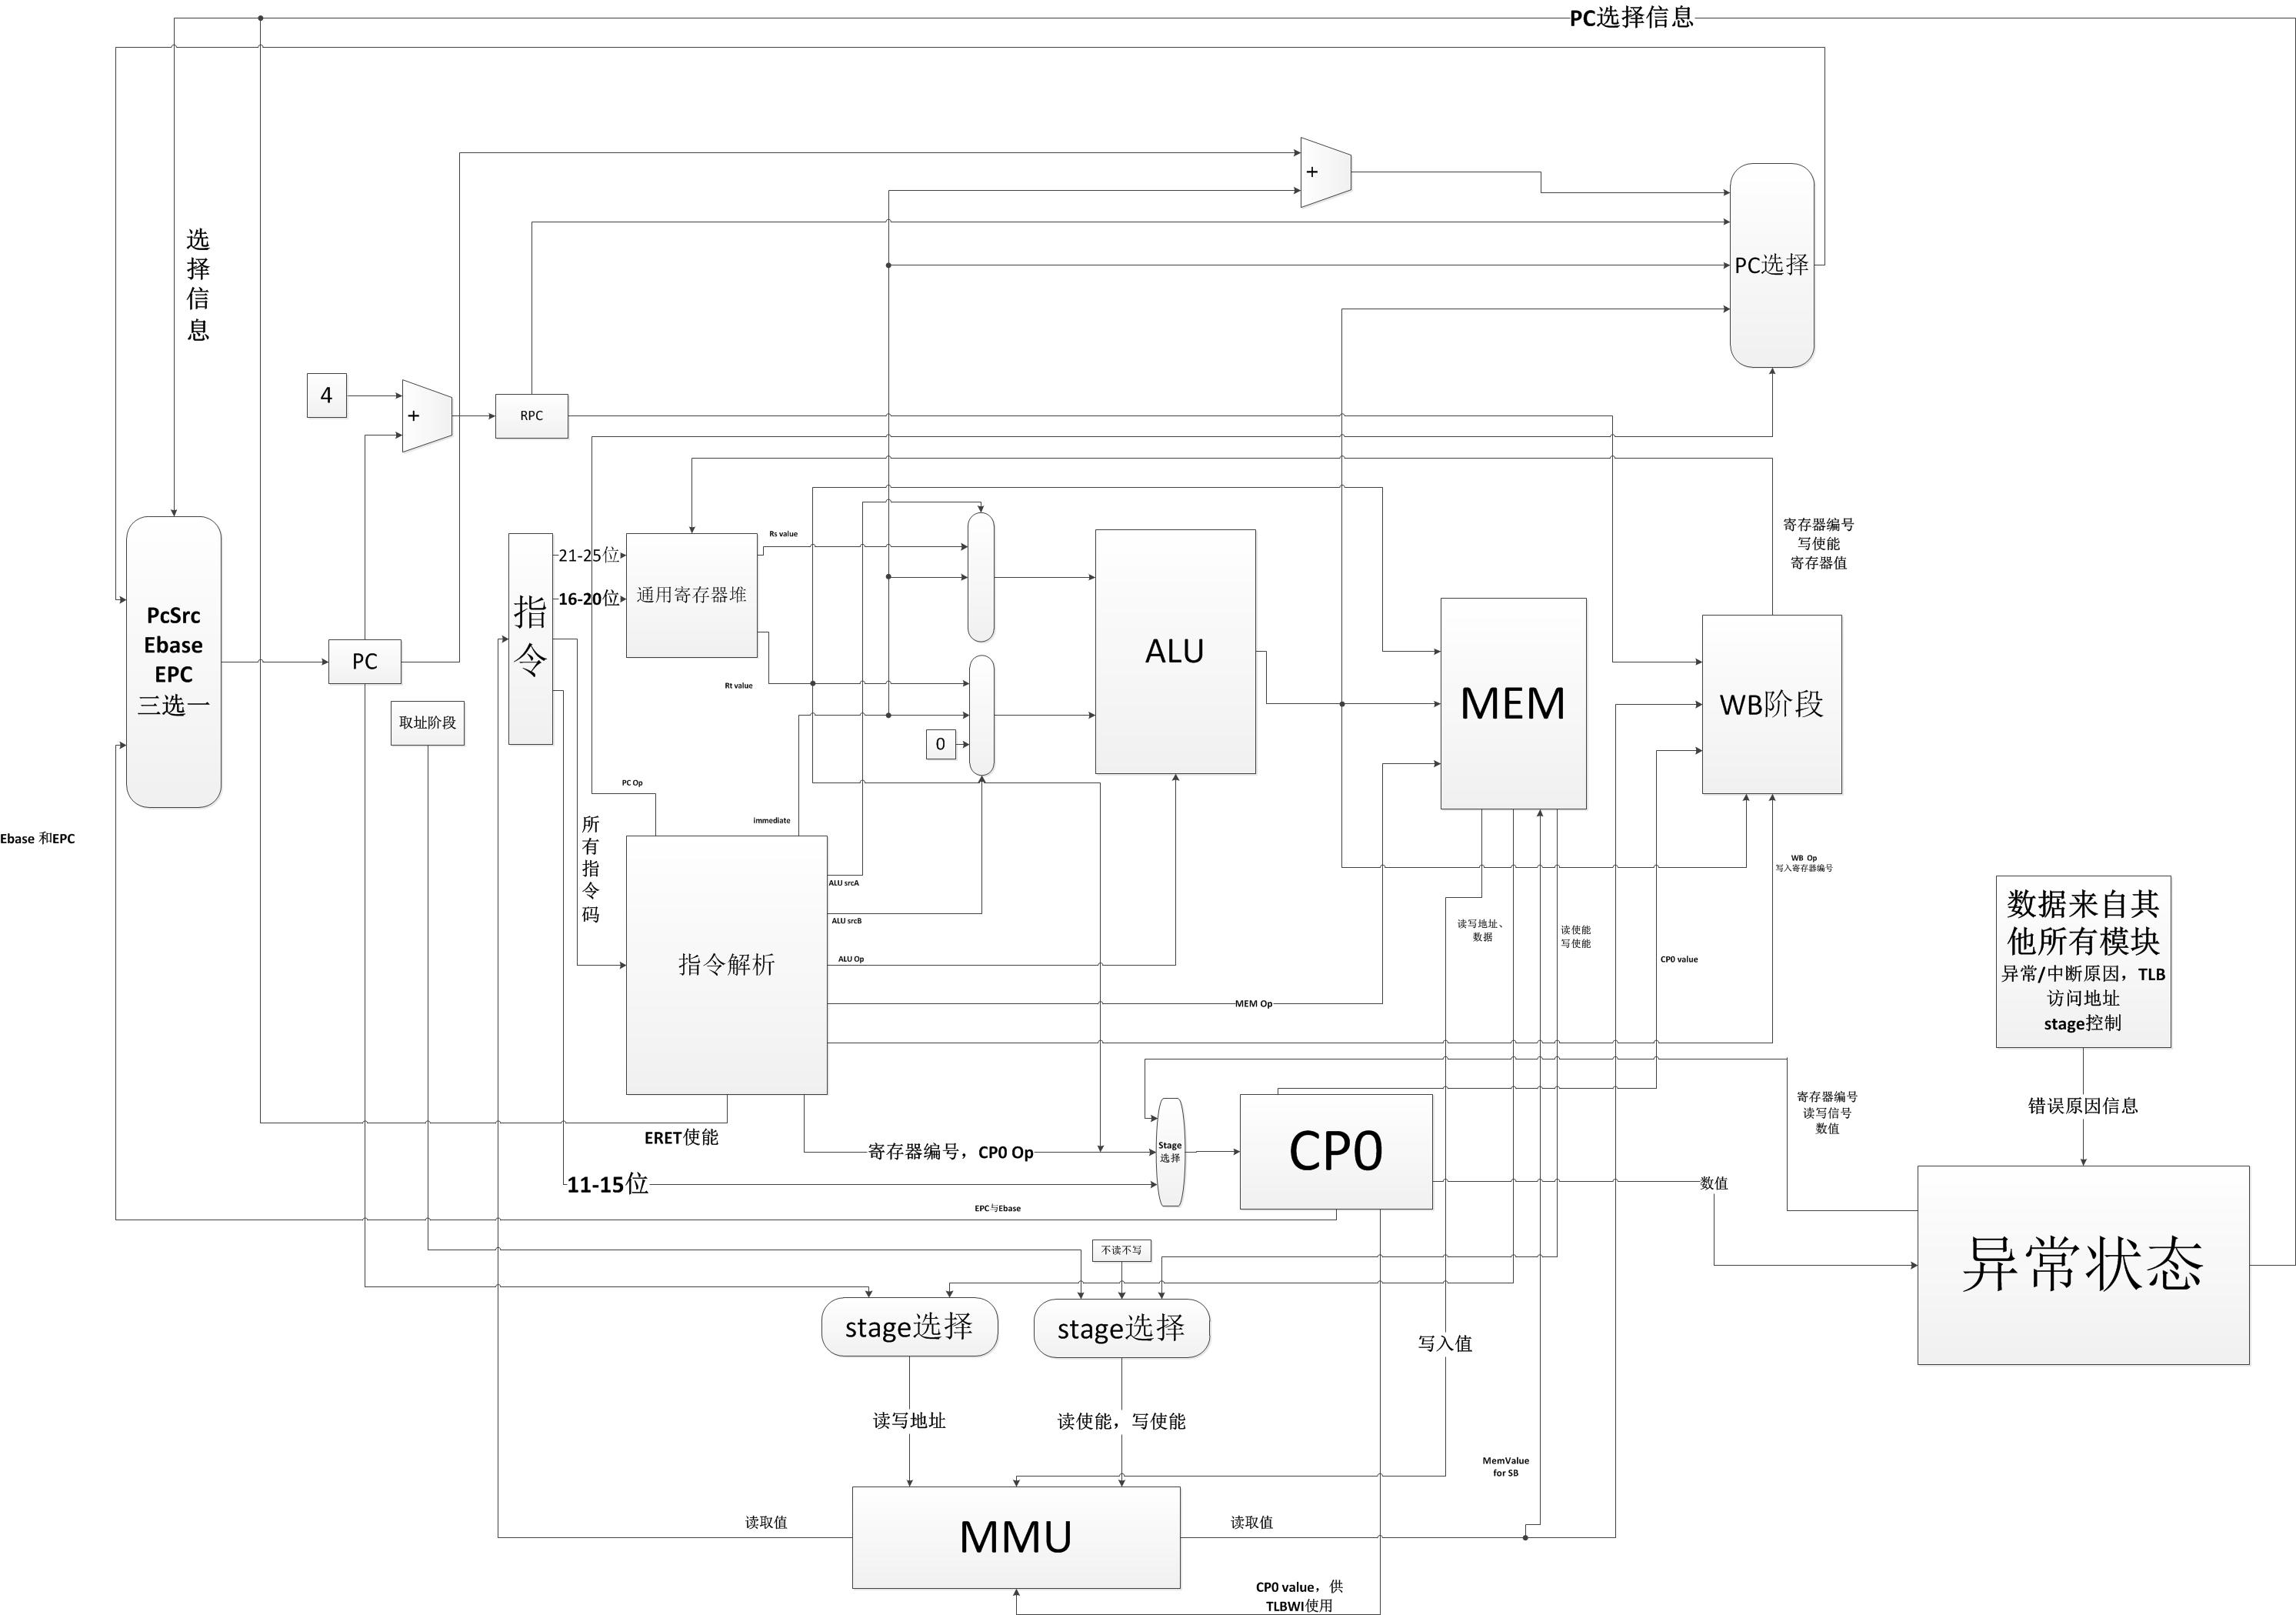
\includegraphics[width=0.9\textwidth]{chart/CPU.jpg}
        \end{figure}

    \subsection{元件例化}
        CPU顶层主要的功能为实现例化各个单独模块并进行模块间的互联。
        按照CPU整体设计图,
        元件例化每个在模块设计部分所出现的模块,
        各个模块间的连接线由模块设计部分给出。

    \subsection{其他实现}
        除元件例化外,CPU顶层还需实现的功能为主状态机的跳转、
        时钟分频以及异常信息的处理。

        \subsubsection{状态机跳转}
            CPU顶层需要实现主状态机的跳转。

            与状态机跳转相关的信号有五个,
            以下分别对其功能进行说明

            \begin{tabularx}{\textwidth}{lll}
                \toprule
                信号名          & 信号类型  & 信号简介 \\
                \cmidrule(l){2-3}
                &
                \multicolumn{2}{X}{信号描述} \\
                \midrule
                has\_mem1             & std\_logic        & 是否有第一访存周期 \\
                \cmidrule(l){2-3}
                &
                \multicolumn{2}{X}{
                    由于对PC的修改在WriteBack阶段进行,
                    因此每条指令都必须有写回阶段。
                    为简化实现,也迫使每条指令都有执行阶段,
                    不需要使用ALU的指令在此阶段不做任何操作。

                    在指令解码的时钟上升沿对指令进行分类,对需要进行访存的指令,
                    has\_mem1置1,表示有访存阶段。其他不涉及到访存指令的has\_mem置0
                } \\
                \midrule
                has\_mem2             & std\_logic        & 是否有第二访存周期 \\
                \cmidrule(l){2-3}
                &
                \multicolumn{2}{X}{
                    专门为SB指令设计,判断是否有第二访存周期。
                    仅当指令为SB时has\_mem2置1,其他情况置0
                } \\
                \midrule
                old\_state             & status        & 访存保持状态 \\
                \cmidrule(l){2-3}
                &
                \multicolumn{2}{X}{
                    CPU对Ram、Flash、串口的访问进行了统一的封装,
                    因此一次访存的时间可能超过一个时钟周期。
                    old\_state用来在访存时间超过一个时钟周期时,
                    保持访存的状态不变。
                } \\
                \midrule
                next\_state             & status        & 下一状态 \\
                \cmidrule(l){2-3}
                &
                \multicolumn{2}{X}{
                    表示当前状态的下一状态。
                    由于执行和写回阶段是每条指令必须经过的阶段,
                    因此只通过has\_mem1和has\_mem2两个信号,
                    对是否有访存阶段进行选择。

                    该信号通过时序逻辑进行控制,每个时钟上升沿根据state进行变化。
                } \\
                \midrule
                state             & status        & 当前状态 \\
                \cmidrule(l){2-3}
                &
                \multicolumn{2}{X}{
                    CPU状态机的当前状态,
                    可能的取值为old\_state或者next\_state或者为异常状态。
                    该信号通过组合逻辑进行控制。

                    在访存过程中,访存的busy信号持续为1,此时state保持为old\_state,
                    保证一次访存结束之后,CPU主状态机再继续跳转。

                    如果有异常信号被置1,则state变为异常状态。
                    之后由异常处理模块保存异常信息,跳转到异常处理向量,
                    再次进行取指令操作。

                    其他状态下,state被赋值为next\_state,
                    表示正常情况下的状态跳转。
                } \\
                \bottomrule
            \end{tabularx}

        \subsubsection{异常处理}
            CPU顶层收集来自各个模块的异常信息,用来判断状态跳转,
            其他异常相关工作交给异常处理模块负责。

            与异常处理相关的信号有三个,
            一下分别对其功能进行说明。

            \begin{tabularx}{\textwidth}{lll}
                \toprule
                信号名          & 信号类型  & 信号简介 \\
                \cmidrule(l){2-3}
                &
                \multicolumn{2}{X}{信号描述} \\
                \midrule
                clock\_inter\_to\_excep   & std\_logic    & 时钟中断信号 \\
                \cmidrule(l){2-3}
                &
                \multicolumn{2}{X}{
                    初始的时钟中断信号由CP0模块产生,
                    当CP0中status寄存器的EXL位为0时,中断有效。

                    同时,由于外部中断并不需要在产生的时候立刻被处理,
                    因此我们选择在写回阶段,对中断信号进行判断,
                    保证这一条指令正常执行完毕后,
                    再对时钟中断进行处理。
                } \\
                \midrule
                serial\_inter\_to\_excep   & std\_logic    & 串口中断信号 \\
                \cmidrule(l){2-3}
                &
                \multicolumn{2}{X}{
                    初始的串口中断信号由访存模块产生。
                    其他处理方式与时钟中断相同。
                } \\
                \midrule
                excep   & std\_logic    & 异常中断信号 \\
                \cmidrule(l){2-3}
                &
                \multicolumn{2}{X}{
                    表明是否发生异常或中断,
                    用来决定CPU主状态机的跳转。

                    正常情况下所有模块发送来的异常信号均为0,
                    因此将所有异常位做逻辑或,
                    即为excep信号。
                } \\
                \bottomrule
            \end{tabularx}

        \subsubsection{时钟分频}
            访存模块始终工作在$25MHz$的高频下,
            分频后得到CPU时钟的工作频率。
    
            CPU单独运行时采用四分频,工作在$6.25MHz$。
            调试模式下,需要再次将时钟分频进行控制,
            此时CPU工作在$3.125MHz$。
